%%%%%%%%%%%%%%%%%%%%%%%%%%%%%%%%%%%%%%%%%%%%%%%%%%%%%%%%%%%%%%%%%%%%%%%%%%%%%%%%%%%%%%%%%
\section{A Survey of WEC Reliability, Survival and Design Practices}
%%%%%%%%%%%%%%%%%%%%%%%%%%%%%%%%%%%%%%%%%%%%%%%%%%%%%%%%%%%%%%%%%%%%%%%%%%%%%%%%%%%%%%%%%
A number of standards/technical specifications (TS) can be considered for WEC design.
An even larger number of informal guidelines and best-practices documents are available on the subject, with yet more standards, guidelines and other documents available on related systems, such as ships and offshore structures.
However, IEC TS 62600-2 (\cite{IECTS62600-2}) is currently the only standard/TS dedicated specifically to WEC design.
This TS gives design guidance for WECs, as well as current energy converters (CECs) and tidal energy converters (TECs).
In addition to IEC TS 62600-2, a number of documents for offshore structures can also provide useful guidance.
N-003 (\cite{N-003}) is the NORSOK % not an acronym
offshore structure design standard; DNV-RP-C205 (\cite{DNV-RP-C205}) is a Det Norkse Veritas (DNV) recommended practices document targeted at offshore structures ; American Bureau of Shipping (\cite{ABS2011}), DNV (\cite{DNV-OS-J101}) and IEC (\cite{IEC61400-3}) all have design documents for offshore wind turbines.

Following an initial review of extreme conditions modeling and design response analysis practices (\cite{Coe2014a}), the study provides a review and general survey of design practices for WECs, by examining the key components of the WEC design process.
We summarize the general stages and workflow for wave energy converter design, relying on supporting articles to provide insight.
A generalized workflow diagram is shown in \figurename~\ref{fig:WecDesignWorkflow}.
Working from left to right, this diagram illustrates a major steps in determining characteristic loads for a WEC.
This characteristic load, which may be the maximum mooring tension or equivalent fatigue load in a structural member, can be evaluated against structural capacities.
The workflow blocks in \figurename~\ref{fig:WecDesignWorkflow} (design framework selection, device configurations, failure modes analysis, environmental characterization, modeling, experimental testing, extreme response statistics and fatigue analysis) are considered in turn.
More details for each of these areas/blocks were described by \cite{Coe2017}, including some general discussion of relevant methods, studies applying these methods for WECs and related systems that were considered.

\begin{figure}[H]
	\centering
	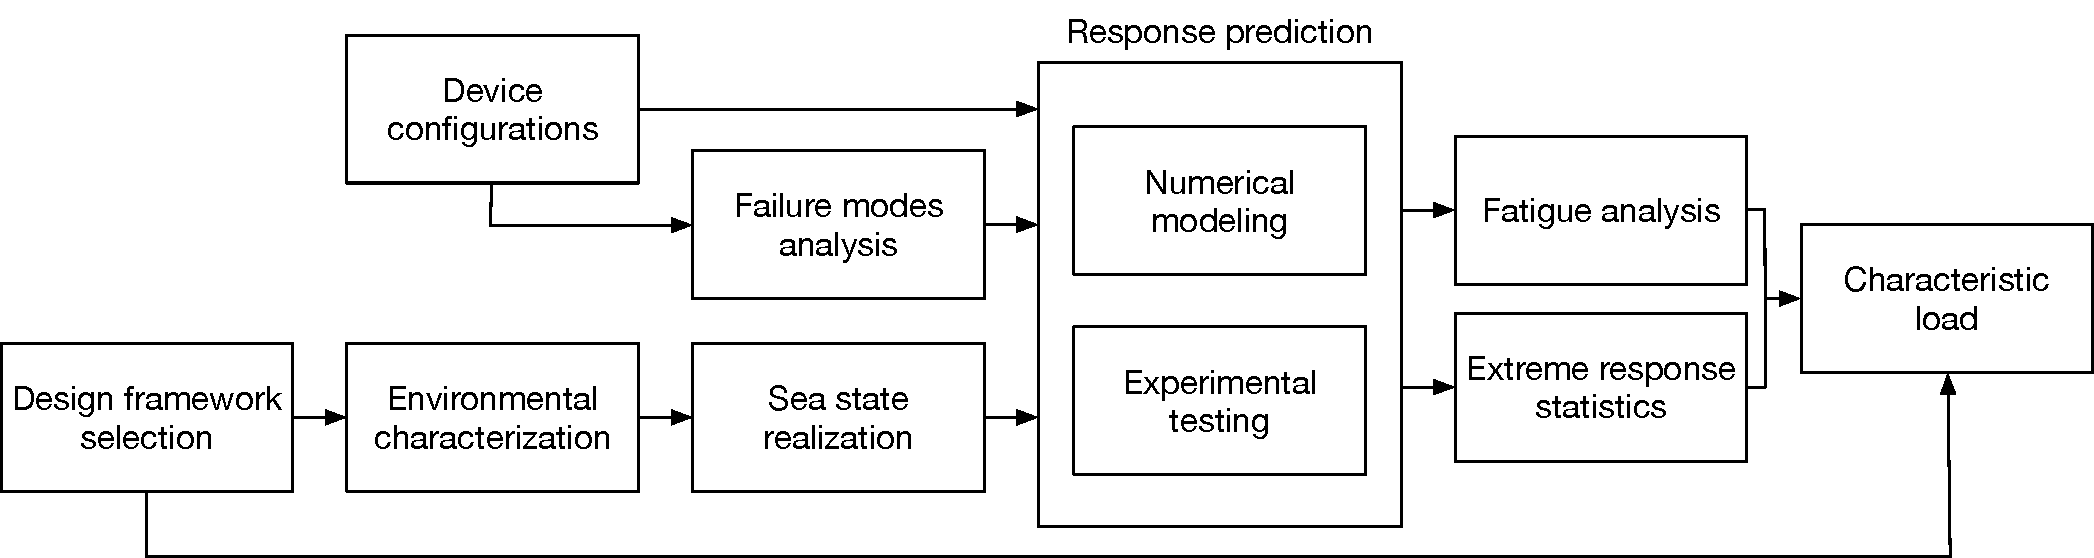
\includegraphics[width=0.96\textwidth]{./Figures/WecDesignWorkflow.pdf}
	\caption{General WEC design workflow with component processes.}
	\label{fig:WecDesignWorkflow}
\end{figure}




%%%%%%%%%%%%%%%%%%%%%%%%%%%%%%%%%%%%%%%%%%%%%%%%%%%%%%%%%%%%%%%%%%%%%%%%%%%%%%%%%%%%%%%%%
